\documentclass{standalone}
\usepackage{graphicx}	
\usepackage{amssymb, amsmath, amsthm}
\usepackage{color}

\usepackage{tikz}
\usetikzlibrary{intersections, backgrounds}

\definecolor{light}{RGB}{179, 255, 255}
\definecolor{light_highlight}{RGB}{154, 246,255}
\definecolor{mid}{RGB}{103,195,255}
\definecolor{mid_highlight}{RGB}{52,144,204}
\definecolor{dark}{RGB}{1,93,153}
\definecolor{dark_highlight}{RGB}{0,42,102}
\definecolor{gray10}{gray}{0.1}
\definecolor{gray20}{gray}{0.2}
\definecolor{gray30}{gray}{0.3}
\definecolor{gray40}{gray}{0.4}
\definecolor{gray60}{gray}{0.6}
\definecolor{gray70}{gray}{0.7}
\definecolor{gray80}{gray}{0.8}
\definecolor{gray90}{gray}{0.9}
\definecolor{gray95}{gray}{0.95}


\begin{document}

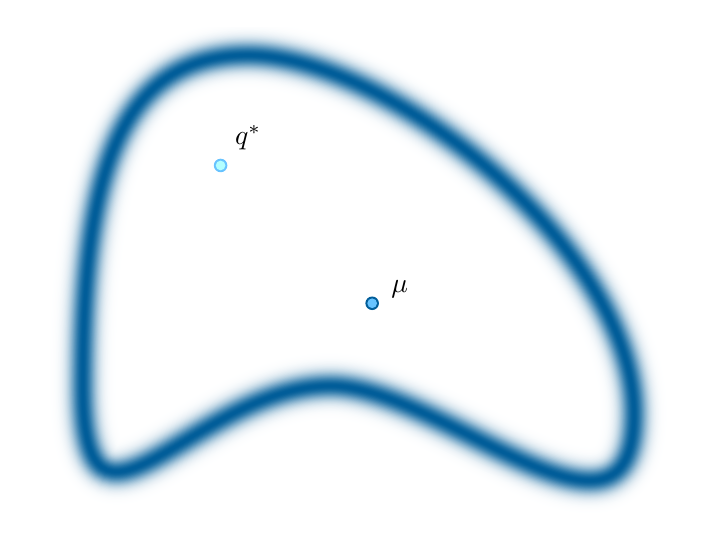
\begin{tikzpicture}[scale=0.35, thick]

    \begin{scope}
        \clip (-12, -7) rectangle (12, 11);
        \foreach \i in {1, 0.99, ..., 0} {
                \pgfmathsetmacro{\prop}{100 * exp(-10.0 * \i * \i)};
                \colorlet{custom}{dark!\prop!white};
                \draw[line width={30
                            * \i}, color=custom]
                (-10, -2) .. controls (-10, 5) and (-9, 10) .. (-4, 10)
                .. controls (1, 10) and (10, 3) .. (10, -3)
                .. controls (10, -9) and (3, -2) .. (-1, -2)
                .. controls (-6, -2) and (-10, -9) .. (-10, -2);
            }
    \end{scope}

      \fill[color=mid] (-5, 6) circle (7pt);
      \fill[color=light] (-5, 6) circle (5pt);
      \node[] at (-4, 7) {$q^*$};   

      \fill[color=dark] (0.5, 1) circle (7pt);
      \fill[color=mid] (0.5, 1) circle (5pt);
      \node[] at (1.5, 1.5) {$\mu$};   



\end{tikzpicture}


\end{document}